\documentclass{article}

\usepackage{graphicx}

\title{Distributed Version Control Systems}

%\author{
% \IEEEauthorblockN{Daniel Persson}
% \IEEEauthorblockA{daniel@silvertejp.org} \and
%
% \IEEEauthorblockN{Olof Johansson}
% \IEEEauthorblockA{olof@ethup.se}
%}
%
%\IEEEpubid{0000--0000/00\$00~\copyright~2011}
%
\begin{document}

\maketitle

\begin{abstract}
 Place abstract here.
\end{abstract}

%\begin{IEEEkeywords}
% Version Control, Configuration Management
%\end{IEEEkeywords}

\section{Introduction}

\section{Background}
%
%\subsection{The History of Version Control}
%The history of Version Control Systems can be divided into three
%categories; the ones that only manages local files, the ones that rely
%on a central server to serve connecting clients, and finally the
%distributed ones, where every 'node' can act as both a client and a
%server. The three categories roughly follow each other
%chronologically, naturally with transition-periods in between. At the
%moment the dominating tools are mostly client-server, but the
%distributed ones are rising fast in popularity, so perhaps we are
%currently in the start of a new transition.
%
%\subsubsection{The Local Era}
%The first VCS ever released was the \emph{Source Code Control System}
%(SCCS) in 1972. SCCS tried to solve a number of problems that software
%developers of that time had. Manually managing several versions of the
%same product simultaneously was not feasible in the long run for
%several reasons described by the creator of SCCS, Marc J. Rochkind
%\cite{sccs}:
%
%\begin{itemize}
% \item The amount of space to store the source code may be several
%       times that needed for any particular version.
% \item Fixes made to one version sometimes fail to get made to
%       other versions.
% \item When changes occur it is difficult to tell exactly what changed
%       and when.
% \item When a customer has a problem it is hard to figure out what
%       version he has.
%\end{itemize}
%
%Instead of saving entire files in various states, SCCS stores the
%differences between versions of the same file (called diffs, or
%deltas). With each delta SCCS also stores metadata such as who made
%the change, why, and when. This did not only save precious storage
%space, but also provided the \emph{traceability} that the software
%developers had previously lacked.
%
%It is worth noting that SCCS was not the only VCS that followed the
%philosophy of storing the files locally, \emph{Revision Control
%  System} (RCS) was released in 1982 and gradually took over as the
%dominant VCS for Unix.
%

\subsection{VCS Workflow}

VCS can be used in a number of ways. Some limits are posed by the choice
of tools. Subversion is built for centralized version control, whereas
tools like git or mercurial are built for decentralized. Members of the 
latter category are generally more flexible; e.g. git is almost as simple 
to run centralized as running it decentralized as it is intended. The 
Telia Smart Home project has chosen to use git. The reasons for this are
several: the ability to use git decentralized as well a centralized was a
major point. Also, the prior experience from some members of the project
made the transition for other members less burdensome.

But defining a workflow does not end with selecting a tool. As stated, 
git is very flexible in the way developers interact with it. It is not
uncommon to use it centralized, and in fact, the Telia Smart Home project
does just this in their documentation repository. But one of the key 
strength is its decentralization. It has no enforced "central repository"
through which all changesets must pass. If the team want to have a 
centralized repository it must itself give a arbitrary repository that
semantic meaning.

Are there any alternatives to be considered? Certainly. Again, git is 
indeed quite flexible. It will yield to the wishes of the user. There are 
a number of easily recognized workflows (perhaps not always mutually
exclusive). Some of the most popular ones are presented here:

\begin{itemize}
 \item \textbf{Centralized}: 
	Using git in a way similar to e.g. Subversion or other more traditional
	tools still give the user some advantages. The process of branching and
	merging is many times more well developed in git than it is in tools like
	Subversion. A property of the distributed nature of git gives yet another
	benefit: having all of the history available locally. You don't need
	network to be able to see what changes was introduced to a particular
	commit, and indeed no network to be able to see the commit log.

 \item \textbf{Topic branches}: 
  Working on a new cool, but experimental feature? Perhaps it is not as 
  tested as the rest of the system is. You probably don't want to have 
  it in the main code. Create a branch specifically for this "topic" or
  "feature".

 \item \textbf{Benevolent dictator}: 
  A workflow, especially popular within open source projects, is the
  benevolent dictator workflow. There is one designated maintainer, and
  other contributers make "pull requests", primarily via e-mail.  If the
  benevolent dictator accepts the patch, he or she merges it into his or
  hers own repository, where everybody gets their source code from. The
  name, "Benevolent dictator", is a term jokingly used about Linus
  Torvalds, the initial author and later primary maintainer for the Linux
  kernel (and also, the initial author of git!).
\end{itemize}

\begin{figure}
 \begin{center}
  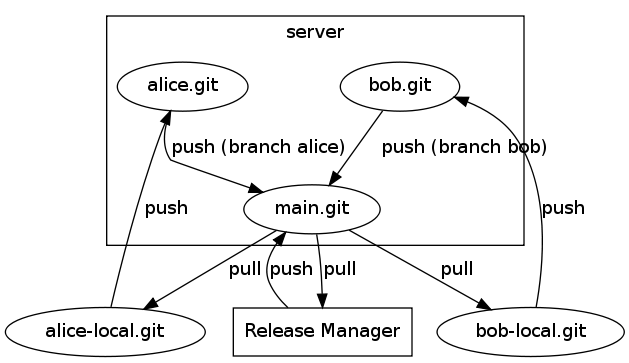
\includegraphics[width=\textwidth]{workflow.png}
  \caption{Workflow description}
  \label{fig:workflow}
 \end{center}
\end{figure}

Each of these workflows are appropriate in some situations. However,
none of these totally fitted the needs of the Telia project. Instead,
the Telia Smart Home project designed its own workflow (see Figure
\ref{fig:workflow}). The workflow used for the code repositories in the
project is based upon individual developer repositories and branches.
Each developer has an own repository, and makes commits to this. The
system (with the help of so called hooks (i.e. scripts triggered by
specific events)) then pushes changes to a repository on a central build
server. Here, a build is triggered using the \emph{Jenkins} continuous
integration system and the commit is also forwarded to the so called
"baseline" repository, but only to a developer's private branch. It is
not merged into the actual baseline code, but it is still accessible for
other developers.

The release manager is now notified that there is a commit awaiting
approval. He or she can check build and test status on Jenkins and see the
delta between baseline and the proposed patch. After possibly running local
tests, the release manager can either approve and merge the commit or
reject it, and inform the author of why it wasn't suitable for inclusion.
If the commit is merged, other developers are now encouraged to merge it 
into their local repositories, their working copy of the source code. 

When designing this system, the sought benefits was the integrated code 
review and approval system. With this, the release managers could validate 
adherence to coding conventions as well as making sure that the system
is buildable and all unit tests passes. Possibly, much of this could even
have been automated (e.g. static code analysis and coding style validation
tools are commonplace) to an even higher degree, but that is, as always, a 
cost/benefit question. It is innovative and unique, but it does build upon
the so called "benevolent dictator" workflow, especially the release
management component of it. The success of this workflow from high-profile 
projects like the Linux kernel has been an inspiration for the design.
The reason why the project rejected the topic branch workflow at an early
stage was the problems associated with topic branches in the early stages
of a software project, where a lot of interdependencies exist and basic
infrastructure is needed. In later stages of the project, this workflow
would have been more feasible, but the overhead associated with switching
workflow was deemed to high. It has been used in some rare cases, where code
was at a very experimental stage.

\section{Research Methodology}

\subsection{Research Questions}
Given the description in the background we intend to investigate the
benefits and drawbacks of using that workflow. To tackle these issues
we have identified the following research questions:

\begin{itemize}
 \item How do the developers adapt to the workflow described above?
 \item How does the workflow affect code quality in relation to the
       release management and code review?
\end{itemize}

By code quality we mean both adherence to the Coding Convention and
error frequency, specifically build and automatic unit-test errors.

\subsection{Research Methodology}
To answer the questions we will conduct both a review of literature in
the field of configuration management in general, and version control
systems in particular, and then conduct a post-mortem analysis of the
project. The primary means of doing the post-mortem analysis will be
to conduct interviews with participants in their various roles. In
addition to this we will also collect data from various project
management and configuration management tools and systems.

\subsubsection{Literature Review}
\label{sec:litreview}

\subsubsection{Post-mortem Analysis}
The post-mortem analysis will primarily be based on interviews with
participants in the Telia Smart Home project and questionnaries with
members from other projects within the same course framework. We will
base the interviews and questionnaries around these questions:

\begin{itemize}
 \item How would you rate your previous experience in using Version Control 
       Systems?
 \item How would you rate your proficiency in using Version Control Systems?
 \item What benefits do you see in using this workflow?
 \item What drawbacks do you see in using this workflow?
 \item Do you have any suggestions for improvements?
 \item What is your overall opinion of the workflow?
\end{itemize}

The post-mortem analysis will also include an analysis of various data
collected during the project. Most of this data will come from
different configuration and project management tools, such as Git for
Version Control, Jenkins for continuous integration and Redmine for
time management and issue tracking.

From Git we will extract metadata related to each commit, such as
time, size, author and commit messages, Jenkins can produce data on
build and test errors, and from Redmine we will compile reports
related to time spent on release management.

The data collected from the project and configuration management tools
will then be correlated with the data gained from the interviews and
questionnaries.

\section{Results of literature study}

\begin{center}
 \emph{Please note: This is a preliminary report on the findings. The format
       of this will change.}
\end{center}

Using the search strategies as described in Section \ref{sec:litreview}, 
we have found a number of relevant published articles and conference 
papers.  The search tools used, primarily Google Scholar, is designed to 
display decreasingly relevant matches. To list all articles we found 
using the search strings is deemed unfeasible. We will therefore limit 
ourselves to describe the selected articles. We have, as stated under
Section \ref{sec:litreview}, constrained the search to the configuration
management domain, and specifically papers either describing details of
version control system workflows, version control system concepts or
configuration management practices relating to version control (explicitly
as well as implicitly). This somewhat wide search domain was a result of the
lack of papers dealing exclusively and explicitly with distributed version 
control workflows. The following papers are a result of this search. We
have dismissed a number of papers after concluding that they fall outside of
the domain. 

\subsection{Selected Papers}
\subsubsection{Version Management Tools: CVS to BK in the Linux Kernel}

An article by M. Shaikh and T. Cornford, written in 2002 and published 
in 3rd Workshop on Open Source Software Engineering\cite{shaikh02}.

\begin{abstract}
 Version management tools might be seen as a prerequisite for open
 source development today as projects become too large to be managed by
 maintainers alone. Yet the OS\footnote{ 
  OS, as in Open Source. Not to be confused with Operating System, our 
  comment.
 } process depends on fluid coordination and collaboration with the
 underlying qualities of this process based on firm trust and
 respect for fellow developers. This paper is a study of how
 debate over version tools reflects governance and decision making
 in an OS community. The paper is based on a study of the Linux kernel
 community as it first saw a partial acceptance of the CVS tool, and then
 later adopted BK\footnote{
  Bitkeeper, a proprietary version control system, our comment. 
 }. The paper explains the adoption process in relation to governance
 concerns, license issues, and questions of technical performance.
\end{abstract}

The described problems with introducing a distributed version control
system into a such a large project as the Linux kernel, may give us 
insight into the adaption process.

\subsubsection{Making Sense of Revision-Control Systems}

An article by B. O'Sullivan, written in 2009 and published in
Communications of the ACM\cite{osullivan09}.

\begin{abstract}
 All revision-control systems come with complicated sets of trade-offs. How
 do you find the best match between tool and team?
\end{abstract}

A high-level description of revision control tools and concepts and its use
will give us a reference on what properties is interesting in version
control workflows.

\subsubsection{Darcs: Distributed Version Management in Haskell}

An article by D. Roundy, written in 2005 and published in Proceedings of the
2005 ACM SIGPLAN workshop on Haskell\cite{roundy05}.

\begin{abstract}
 A common reaction from people who hear about darcs, the source control
 system I created, is that I sounds like a great tool, but it is a shame
 that it is written in Haskell. People think that because darcs is written
 in Haskell it will be a slow memory hog with very few contributors to the
 project. I will give a somewhat historical overview of my experiences with
 the Haskell language, libraries and tools.

 I will begin with a brief overview of the darcs advanced revision control
 system, how it works and how it differs form other version control systems.
 Then I will go through various problems and successes I have had in using
 the Haskell language and libraries in darcs, roughly in the order I
 encountered them. In the process I will give a bit of a tour through the
 darcs source code. In each case, I will tell about the problem I wanted to
 solve, what I tried, how it worked, and how it might have worked better (if
 that is possible).
\end{abstract}

A case study into a specific distributed version control system. Even though
the paper deals in large parts with the implementation details, the actual
usage and interaction with the system is described.

\subsubsection{Towards a Better SCM: Revlog and Mercurial}

An article by M. Mackall, written in 2006 and published in the Linux
Symposium\cite{mackall06}.

\begin{abstract}
 Large projects need scalable, performant, and robust software configuration
 management systems. If common revision control operations are not cheap,
 they present a large barrier to proper software engineering practice. This
 paper will investigate the theoretical limits on SCM performance, and
 examines how existing systems fall short of those ideals.

 I then describe the Revlog data storage scheme created for the Mercurial
 SCM. The Revlog scheme allows all common SCM operations to be performed in
 near-optimal time, while providing excellent compression and robustness. 

 Finally, I look at how a full distributed SCM (Mercurial) is built on top
 of the Revlog scheme, some of the pitfalls we've surmounted in on-disk
 layout and I/O performance and the protocols used to efficiently
 communicate between repositories.
\end{abstract}

Yet another case study into a specific distributed version control system.
Again, this also deals with technical details, but the interaction and usage
pattern is interesting for our research.

\subsubsection{The Promises and Perils of Mining Git}

An article by C Bird, P. C. Rigby, E. T. Barr, D. J. Hamilton, D. M. German
and P Devanbu, written in 2009 and published in 2009 6th IEEE International 
Working Conference on Mining Software Repositories\cite{bird09}.

\begin{abstract}
 We are now witnessing the rapid growth of decentralized source code
 management (DSCM) systems, in which every developer has her own repository.
 DCSMs facilitate a style of collaboration in which work output can flow
 sideways (and privately) between collaborators, rather than always up and
 down (and publicly) via a central repository. Decentralization comes with
 both the promise of new data and the peril of its misinterpretation. We
 focus on git, a very popular DSCM used in high-profile projects.
 Decentralization, and other features of git, such as automatically recorded
 contributor attribution, lead to richer content histories, giving rise to
 new questions such as "How do contributions flow between developers to the
 official project repository?" However, there are pitfalls. Commits may be
 reordered, deleted, or edited as they move between repositories. The
 semantics of terms common to SCMs and DSCMs sometimes differ markedly,
 potentially creating confusion. For example, a commit is immediately
 visible to all developers in centralized SCMs, but not in DSCMs. Our goal
 is to help researchers interested in DSCMs avoid these and other perils
 when mining and analyzing git data.
\end{abstract}

And a third (and final) case study into a specific version control system.
This paper does not primarily deal with technical details however, and
instead focusing on interaction details. 

\subsubsection{Why Are Software Projects Moving From Centralized to
               Decentralized Version Control Systems?}

An article by D. de Alwis and J. Sillito, written in 2009 and published in 
2009 ICSE Workshop on Cooperative and Human Aspects on Software
Engineering\cite{alwis09}.

\begin{abstract}
 Version control systems are essential for co-ordinating work on a software
 project. A number of open- and closed-source projects are proposing to
 move, or have already moved, their source code repositories from a
 centralized version control system (CVCS) to a decentralized version
 control system (DVCS). In this paper we summarize the differences between a
 CVCS and a DVCS, and describe some of the rationales and perceived benefits
 offered by projects to justify the transition.
\end{abstract}

This paper is relevant to us and important for us to understand the reasons
for migration, and as a reference for comparisons with centralized version 
control systems.

\subsubsection{DVCS or a new way to use Version Control Systems for FreeBSD}

An article by O. Robert, written in 2006\cite{robert06}.

\begin{abstract}
 FreeBSD, like many open source projects, uses CVS as its main versioon
 control system (VCS), which is an extended history of all modifications
 made since the beginning of the project in 1993. CVS is a cornerstone of
 FreeBSD in two ways: not only does it record the history of the project,
 but it is a fundamental tool for coordinating the development of the
 FreeBSD operating system.

 CVS is built around the concept of centralised repository, which has a
 number of limitations.

 Recently, a new type of VCS has arisen: Distributed VCS, one of the first
 being BK from BitMover, Inc. Better known from the controversy it generated
 when Linus Torvalds started using it, it has nonetheless changed the way
 some people develop software.

 This paper explores the area of distributed VCS. We analyse two of them
 (Arch in its Bazaar incarnation and Mercuriel and try to show how such a
 tool could help further FreeBSD development, both as a tool and as a new
 development process.\footnote{
  \emph{Sic}, in regards to unbalanced parentheses
 }
\end{abstract}

A paper dealing with a potential migration from a centralized version
control system (CVS), to a decentralized. What would be the benefits for
the FreeBSD project? What would be the drawbacks?

\subsubsection{BitKeeper for Kernel Developers}

An article by V. Henson and J. Garzik, written in 2002 and published in
Ottawa Linux Symposium\cite{henson02}.

\begin{abstract}
 BitKeeper is a revolutionary new distributed source control management
 suite which is ideal for Linux kernel development. BitKeeper provides tools
 which automate and simplify many common kernel development tasks. In this
 paper, we describe basic BitKeeper concepts and operations, BitKeeper
 solutions for common kernel development problems, and a workflow for
 interacting with other Linux developers using BitKeeper. We also discuss
 some of BitKeeper's shortcomings and what is being done to correct them. We
 conclude that BitKeeper can dramatically imrpove the efficiency of Linux
 kernel developers.
\end{abstract}

Bitkeeper is a distributed version control system, and was for a long time
used by the Linux kernel developers for their version control needs. Even
though it was surrounded with controversy, due to its non-free, proprietary
status and hostility against reverse engineering, it was still a major
breakthrough for distributed version control. 

\subsubsection{Software Configuration Management: A Roadmap}

An article by J. Estublier, written in 2000 and published in Proceedings of
the conference on The future of Software engineering\cite{estublier00}.

\begin{abstract}
 This paper, in the first chapter summarizes the state of the art in
 SCM\footnote{
  SCM, as in Software Configuration Management. Not to be confused with
  Source Control Management.
 }, showing the evolution along the last 25 years. Chapter 2 shows the
 current research work under way in the area. In chapter 3, the challenges
 SCM has to take up, as well as SCM future research are discussed.
\end{abstract}

This paper is a general overview of the configuration management field. It
is useful as a basis and context for our research into a specific
configuration management concept and technology, namely version control.

\subsubsection{Learning by Doing: Introducing Version Control as a Way to
               Manage Student Assignments}

An article by K. L. Reid and G. V. Wilson, written in 2005 and published in
ACM SIGCSE Bulletin\cite{reid05}.

\begin{abstract}
 Professional software developers use version control systems to coordinate
 their work, and to provide an unwindable history of their project's
 evolution. In contrast, students in most programming courses use a
 homegrown electronic submission program to submit their work, and email to
 coordinate with partners when doing team projects. In May 2003, we began
 using CVS, a popular open source version control system, as an assignment
 submission system. Students receive starter code by checking out each
 student's repository, and committing the marks. Our experience to date
 shows that this is both a simpler and more flexible way to manage student
 assignments, and also an excellent way to teach them how to use a
 fundamental software development tool.
\end{abstract}

As a large part of our research will be about adaptability and ability to
learn and understand our workflow, it is interesting to see other
experiences within version control education. How did the students adapt to
this somewhat unorthodox assignment submission system?

\bibliographystyle{plain} 
\bibliography{references}

\end{document}
